\documentclass[tikz,border=6pt]{standalone}
% Shared visual language for the original benchmark atlas.
\usepackage[T1]{fontenc}
\usepackage{lmodern}
\usepackage{amsmath,amssymb}
\usetikzlibrary{arrows.meta,calc,positioning,shapes.geometric,patterns,decorations.pathmorphing,backgrounds,fit}
\definecolor{ink}{HTML}{173948}
\definecolor{flow}{HTML}{167D9A}
\definecolor{control}{HTML}{A65217}
\definecolor{measure}{HTML}{70518A}
\definecolor{pale}{HTML}{EAF2F5}
\definecolor{muted}{HTML}{526571}
\definecolor{utility}{HTML}{2E8665}
\tikzset{
  every node/.style={font=\sffamily\small,text=ink},
  equipment/.style={draw=ink,line width=1pt,fill=pale,rounded corners=2pt},
  process/.style={draw=flow,line width=1.2pt,-{Latex[length=2.5mm]}},
  signal/.style={draw=control,line width=.8pt,dashed,-{Latex[length=2mm]}},
  util/.style={draw=utility,line width=1pt,-{Latex[length=2.2mm]}},
  dimension/.style={draw=muted,line width=.6pt,{Latex[length=1.7mm]}-{Latex[length=1.7mm]}},
  labelbox/.style={fill=white,inner sep=2pt,font=\sffamily\footnotesize,align=center},
  annotation/.style={font=\sffamily\footnotesize,text=muted,align=left},
  panel/.style={draw=ink!20,fill=ink!2,rounded corners=3pt,inner sep=6pt},
  instrument/.style={circle,draw=measure,fill=white,line width=.8pt,minimum size=8mm,inner sep=1pt,font=\sffamily\scriptsize,align=center},
  port/.style={circle,fill=flow,inner sep=1.6pt},
  box/.style={equipment,minimum width=3cm,minimum height=1cm,align=center},
}
\newcommand{\atlasheader}[3]{%
  \node[anchor=north west,font=\sffamily\bfseries\LARGE] at (0,0) {#1};%
  \node[anchor=north west,font=\sffamily\small,text=muted] at (0,-.75) {Paper section #2: \textit{#3}};%
  \draw[ink!25,line width=.7pt] (0,-1.25)--(26,-1.25);%
}
\newcommand{\atlasfooter}[1]{%
  \draw[ink!25,line width=.5pt] (0,-15.8)--(26,-15.8);%
  \node[anchor=north west,annotation,text width=25.8cm] at (0,-16) {#1\\Original explanatory drawing. Source: Kroll \& Schulte (2014), DOI: 10.1016/j.asoc.2014.08.034. Model variants are identified in the accompanying case sheet.};%
}

\begin{document}
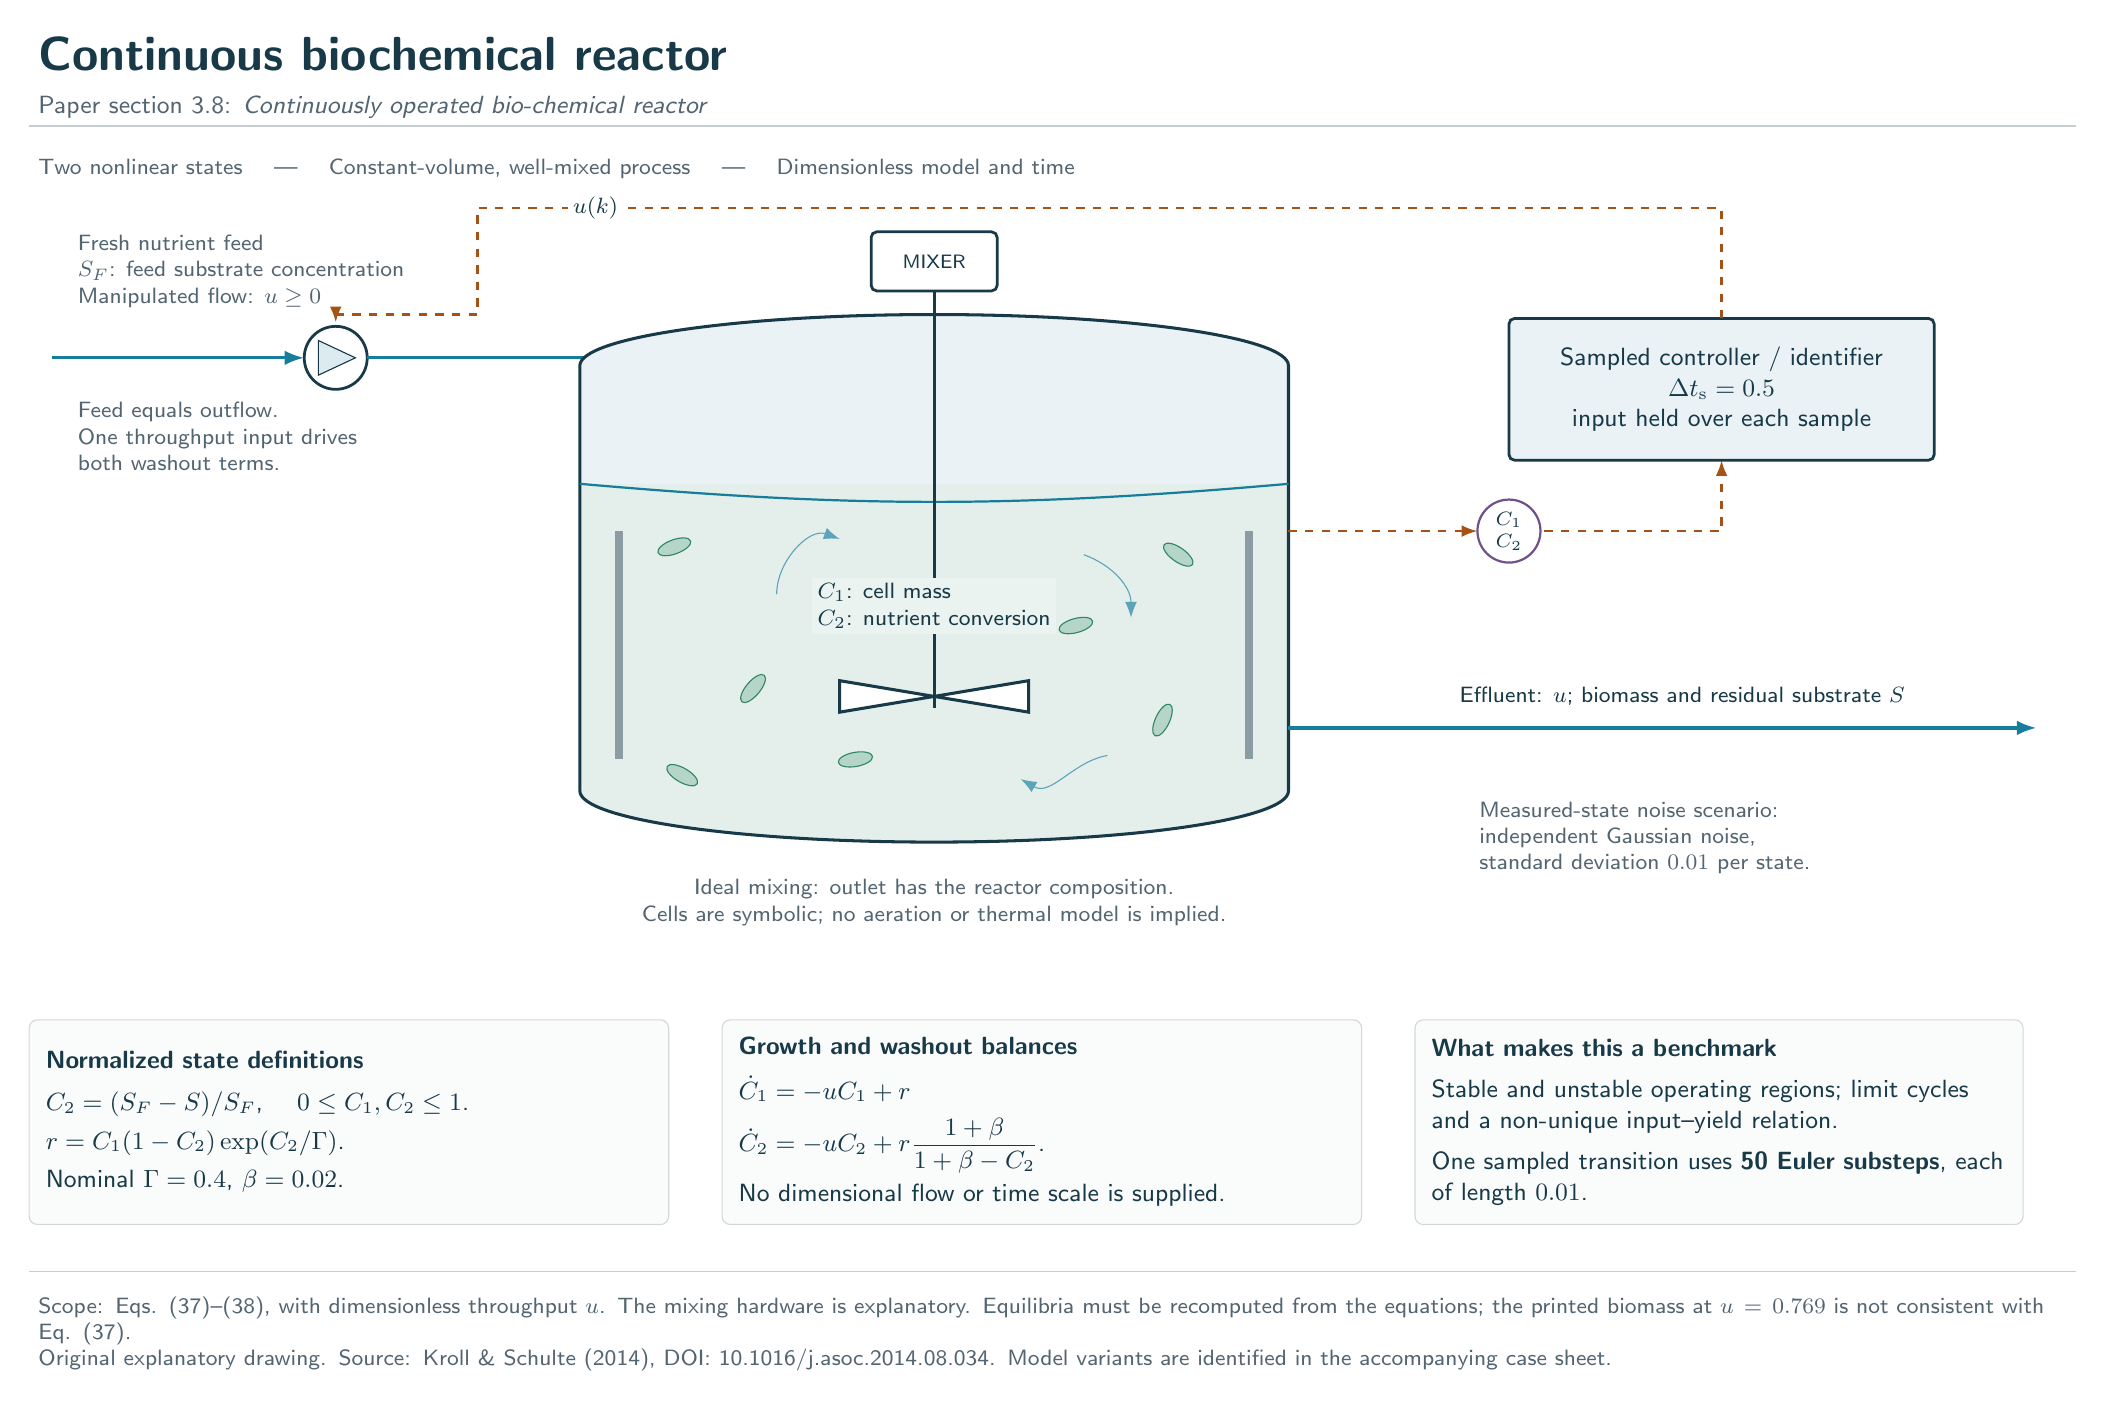
\begin{tikzpicture}[x=1cm,y=1cm]
\atlasheader{Continuous biochemical reactor}{3.8}{Continuously operated bio-chemical reactor}
\node[annotation,anchor=west] at (0,-1.8) {Two nonlinear states \quad | \quad Constant-volume, well-mixed process \quad | \quad Dimensionless model and time};
% Feed and discharge show the single manipulated throughput.
\draw[process] (0.3,-4.2)--(3.5,-4.2);
\draw[equipment,fill=white] (3.9,-4.2) circle[radius=.4];
\draw[ink,fill=flow!15] (3.68,-4.42)--(4.15,-4.2)--(3.68,-3.98)--cycle;
\draw[process] (4.3,-4.2)--(8.5,-4.2)--(8.5,-5.5);
\node[annotation,anchor=west] at (.5,-3.1) {Fresh nutrient feed\\$S_F$: feed substrate concentration\\Manipulated flow: $u\geq0$};
\node[annotation,anchor=west] at (.5,-5.2) {Feed equals outflow.\\One throughput input drives\\both washout terms.};
% Vessel shell, free surface, mixing shaft, baffles and impeller.
\path[fill=pale] (7,-4.3)--(7,-9.7) arc[start angle=180,end angle=360,x radius=4.5,y radius=.65]--(16,-4.3) arc[start angle=0,end angle=180,x radius=4.5,y radius=.65];
\path[fill=utility!13] (7,-5.8)--(7,-9.7) arc[start angle=180,end angle=360,x radius=4.5,y radius=.65]--(16,-5.8)--cycle;
\draw[ink,line width=1.1pt] (7,-4.3)--(7,-9.7) arc[start angle=180,end angle=360,x radius=4.5,y radius=.65]--(16,-4.3) arc[start angle=0,end angle=180,x radius=4.5,y radius=.65];
\draw[flow,line width=.8pt] (7,-5.8) to[out=-5,in=185] (16,-5.8);
\draw[ink!50,line width=3pt] (7.5,-6.4)--(7.5,-9.3) (15.5,-6.4)--(15.5,-9.3);
\draw[equipment,fill=white] (10.7,-2.6) rectangle (12.3,-3.35);
\node[font=\sffamily\scriptsize] at (11.5,-2.98) {MIXER};
\draw[ink,line width=1.2pt] (11.5,-3.35)--(11.5,-8.65);
\draw[ink,line width=1.1pt,fill=white] (10.3,-8.3)--(12.7,-8.7)--(12.7,-8.3)--(10.3,-8.7)--cycle;
\draw[flow!70,-{Latex[length=2mm]}] (9.5,-7.2) to[out=90,in=160] (10.3,-6.5);
\draw[flow!70,-{Latex[length=2mm]}] (13.4,-6.7) to[out=-20,in=90] (14,-7.5);
\draw[flow!70,-{Latex[length=2mm]}] (13.7,-9.25) to[out=190,in=-30] (12.6,-9.55);
% Cell motifs are symbolic biomass, not gas injection.
\foreach \xx/\yy/\ang in {8.2/-6.6/20,9.2/-8.4/50,8.3/-9.5/-30,13.3/-7.6/15,14.4/-8.8/65,10.5/-9.3/10,14.6/-6.7/-35} {
  \draw[utility,fill=utility!35,rotate around={\ang:(\xx,\yy)}] (\xx,\yy) ellipse[x radius=.22,y radius=.09];
}
\node[labelbox,fill=white!90!utility,align=left] at (11.5,-7.35) {$C_1$: cell mass\\$C_2$: nutrient conversion};
\node[annotation,anchor=north,align=center] at (11.5,-10.7) {Ideal mixing: outlet has the reactor composition.\\Cells are symbolic; no aeration or thermal model is implied.};
\draw[process] (16,-8.9)--(25.5,-8.9);
\node[labelbox] at (21,-8.5) {Effluent: $u$; biomass and residual substrate $S$};
% Output and sampled-data feedback make the modeling problem visible.
\draw[signal] (16,-6.4)--(18.4,-6.4);
\node[instrument] at (18.8,-6.4) {$C_1$\\$C_2$};
\draw[signal] (19.25,-6.4)--(21.5,-6.4)--(21.5,-5.5);
\node[box,minimum width=5.4cm,minimum height=1.8cm] at (21.5,-4.6) {Sampled controller / identifier\\$\Delta t_{\mathrm s}=0.5$\\input held over each sample};
\draw[signal] (21.5,-3.7)--(21.5,-2.3)--(5.7,-2.3)--(5.7,-3.65)--(3.9,-3.65)--(3.9,-3.75);
\node[labelbox] at (7.2,-2.3) {$u(k)$};
\node[annotation,anchor=west] at (18.3,-10.3) {Measured-state noise scenario:\\independent Gaussian noise,\\standard deviation $0.01$ per state.};
\node[panel,anchor=north west,text width=7.7cm,minimum height=2.6cm,align=left] at (0,-12.6) {\textbf{Normalized state definitions}\\[4pt]
 $C_2=(S_F-S)/S_F$, $\quad0\leq C_1,C_2\leq1$.\\[3pt]
 $r=C_1(1-C_2)\exp(C_2/\Gamma)$.\\[3pt]
 Nominal $\Gamma=0.4$, $\beta=0.02$.};
\node[panel,anchor=north west,text width=7.7cm,minimum height=2.6cm,align=left] at (8.8,-12.6) {\textbf{Growth and washout balances}\\[5pt]
 $\dot C_1=-uC_1+r$\\[5pt]
 $\displaystyle\dot C_2=-uC_2+r\frac{1+\beta}{1+\beta-C_2}$.\\[3pt]
 No dimensional flow or time scale is supplied.};
\node[panel,anchor=north west,text width=7.3cm,minimum height=2.6cm,align=left] at (17.6,-12.6) {\textbf{What makes this a benchmark}\\[4pt]
 Stable and unstable operating regions; limit cycles and a non-unique input--yield relation.\\[4pt]
 One sampled transition uses \textbf{50 Euler substeps}, each of length $0.01$.};
\atlasfooter{Scope: Eqs. (37)--(38), with dimensionless throughput $u$. The mixing hardware is explanatory. Equilibria must be recomputed from the equations; the printed biomass at $u=0.769$ is not consistent with Eq. (37).}
\end{tikzpicture}
\end{document}
